\documentclass[]{article}
\usepackage{lmodern}
\usepackage{amssymb,amsmath}
\usepackage{ifxetex,ifluatex}
\usepackage{fixltx2e} % provides \textsubscript
\ifnum 0\ifxetex 1\fi\ifluatex 1\fi=0 % if pdftex
  \usepackage[T1]{fontenc}
  \usepackage[utf8]{inputenc}
\else % if luatex or xelatex
  \ifxetex
    \usepackage{mathspec}
  \else
    \usepackage{fontspec}
  \fi
  \defaultfontfeatures{Ligatures=TeX,Scale=MatchLowercase}
\fi
% use upquote if available, for straight quotes in verbatim environments
\IfFileExists{upquote.sty}{\usepackage{upquote}}{}
% use microtype if available
\IfFileExists{microtype.sty}{%
\usepackage{microtype}
\UseMicrotypeSet[protrusion]{basicmath} % disable protrusion for tt fonts
}{}
\usepackage[margin=1in]{geometry}
\usepackage{hyperref}
\hypersetup{unicode=true,
            pdftitle={Math 530/630 CM 5.3},
            pdfborder={0 0 0},
            breaklinks=true}
\urlstyle{same}  % don't use monospace font for urls
\usepackage{color}
\usepackage{fancyvrb}
\newcommand{\VerbBar}{|}
\newcommand{\VERB}{\Verb[commandchars=\\\{\}]}
\DefineVerbatimEnvironment{Highlighting}{Verbatim}{commandchars=\\\{\}}
% Add ',fontsize=\small' for more characters per line
\usepackage{framed}
\definecolor{shadecolor}{RGB}{248,248,248}
\newenvironment{Shaded}{\begin{snugshade}}{\end{snugshade}}
\newcommand{\AlertTok}[1]{\textcolor[rgb]{0.94,0.16,0.16}{#1}}
\newcommand{\AnnotationTok}[1]{\textcolor[rgb]{0.56,0.35,0.01}{\textbf{\textit{#1}}}}
\newcommand{\AttributeTok}[1]{\textcolor[rgb]{0.77,0.63,0.00}{#1}}
\newcommand{\BaseNTok}[1]{\textcolor[rgb]{0.00,0.00,0.81}{#1}}
\newcommand{\BuiltInTok}[1]{#1}
\newcommand{\CharTok}[1]{\textcolor[rgb]{0.31,0.60,0.02}{#1}}
\newcommand{\CommentTok}[1]{\textcolor[rgb]{0.56,0.35,0.01}{\textit{#1}}}
\newcommand{\CommentVarTok}[1]{\textcolor[rgb]{0.56,0.35,0.01}{\textbf{\textit{#1}}}}
\newcommand{\ConstantTok}[1]{\textcolor[rgb]{0.00,0.00,0.00}{#1}}
\newcommand{\ControlFlowTok}[1]{\textcolor[rgb]{0.13,0.29,0.53}{\textbf{#1}}}
\newcommand{\DataTypeTok}[1]{\textcolor[rgb]{0.13,0.29,0.53}{#1}}
\newcommand{\DecValTok}[1]{\textcolor[rgb]{0.00,0.00,0.81}{#1}}
\newcommand{\DocumentationTok}[1]{\textcolor[rgb]{0.56,0.35,0.01}{\textbf{\textit{#1}}}}
\newcommand{\ErrorTok}[1]{\textcolor[rgb]{0.64,0.00,0.00}{\textbf{#1}}}
\newcommand{\ExtensionTok}[1]{#1}
\newcommand{\FloatTok}[1]{\textcolor[rgb]{0.00,0.00,0.81}{#1}}
\newcommand{\FunctionTok}[1]{\textcolor[rgb]{0.00,0.00,0.00}{#1}}
\newcommand{\ImportTok}[1]{#1}
\newcommand{\InformationTok}[1]{\textcolor[rgb]{0.56,0.35,0.01}{\textbf{\textit{#1}}}}
\newcommand{\KeywordTok}[1]{\textcolor[rgb]{0.13,0.29,0.53}{\textbf{#1}}}
\newcommand{\NormalTok}[1]{#1}
\newcommand{\OperatorTok}[1]{\textcolor[rgb]{0.81,0.36,0.00}{\textbf{#1}}}
\newcommand{\OtherTok}[1]{\textcolor[rgb]{0.56,0.35,0.01}{#1}}
\newcommand{\PreprocessorTok}[1]{\textcolor[rgb]{0.56,0.35,0.01}{\textit{#1}}}
\newcommand{\RegionMarkerTok}[1]{#1}
\newcommand{\SpecialCharTok}[1]{\textcolor[rgb]{0.00,0.00,0.00}{#1}}
\newcommand{\SpecialStringTok}[1]{\textcolor[rgb]{0.31,0.60,0.02}{#1}}
\newcommand{\StringTok}[1]{\textcolor[rgb]{0.31,0.60,0.02}{#1}}
\newcommand{\VariableTok}[1]{\textcolor[rgb]{0.00,0.00,0.00}{#1}}
\newcommand{\VerbatimStringTok}[1]{\textcolor[rgb]{0.31,0.60,0.02}{#1}}
\newcommand{\WarningTok}[1]{\textcolor[rgb]{0.56,0.35,0.01}{\textbf{\textit{#1}}}}
\usepackage{longtable,booktabs}
\usepackage{graphicx,grffile}
\makeatletter
\def\maxwidth{\ifdim\Gin@nat@width>\linewidth\linewidth\else\Gin@nat@width\fi}
\def\maxheight{\ifdim\Gin@nat@height>\textheight\textheight\else\Gin@nat@height\fi}
\makeatother
% Scale images if necessary, so that they will not overflow the page
% margins by default, and it is still possible to overwrite the defaults
% using explicit options in \includegraphics[width, height, ...]{}
\setkeys{Gin}{width=\maxwidth,height=\maxheight,keepaspectratio}
\IfFileExists{parskip.sty}{%
\usepackage{parskip}
}{% else
\setlength{\parindent}{0pt}
\setlength{\parskip}{6pt plus 2pt minus 1pt}
}
\setlength{\emergencystretch}{3em}  % prevent overfull lines
\providecommand{\tightlist}{%
  \setlength{\itemsep}{0pt}\setlength{\parskip}{0pt}}
\setcounter{secnumdepth}{0}
% Redefines (sub)paragraphs to behave more like sections
\ifx\paragraph\undefined\else
\let\oldparagraph\paragraph
\renewcommand{\paragraph}[1]{\oldparagraph{#1}\mbox{}}
\fi
\ifx\subparagraph\undefined\else
\let\oldsubparagraph\subparagraph
\renewcommand{\subparagraph}[1]{\oldsubparagraph{#1}\mbox{}}
\fi

%%% Use protect on footnotes to avoid problems with footnotes in titles
\let\rmarkdownfootnote\footnote%
\def\footnote{\protect\rmarkdownfootnote}

%%% Change title format to be more compact
\usepackage{titling}

% Create subtitle command for use in maketitle
\providecommand{\subtitle}[1]{
  \posttitle{
    \begin{center}\large#1\end{center}
    }
}

\setlength{\droptitle}{-2em}

  \title{Math 530/630 CM 5.3}
    \pretitle{\vspace{\droptitle}\centering\huge}
  \posttitle{\par}
  \subtitle{Contrasts, post-hoc tests \& p-value adjustments}
  \author{}
    \preauthor{}\postauthor{}
    \date{}
    \predate{}\postdate{}
  

\begin{document}
\maketitle

\hypertarget{two-key-equations}{%
\section{Two key equations}\label{two-key-equations}}

When I introduced the \emph{t}-test as a general linear model (GLM), I
said that ``all statistical procedures are basically the same thing'':

\[outcome_i=(model)+error_i\]

Where: * Outcome is your dependent variable (DV; also known as \emph{y})
and * Model is a linear function or linear combination of your
independent variable(s) (IVs) (also known as \emph{x}'s)

\[DV_i=(model)+error_i\]

``Essentially, all models are wrong, but some are useful''-George E. P.
Box (1987)

\[deviation=\sum{(observed-model)^2}\]

\begin{center}\rule{0.5\linewidth}{\linethickness}\end{center}

\hypertarget{the-sample-mean}{%
\section{The sample mean}\label{the-sample-mean}}

.pull-left{[} \(DV_i=(1b)+error_i\)

Coefficient=1 is implied. {]}

.pull-right{[} \(DV_i=(model)+error_i\){]}

\begin{center}\rule{0.5\linewidth}{\linethickness}\end{center}

\hypertarget{correlation}{%
\section{Correlation}\label{correlation}}

.pull-left{[}

\(DV_i=(bIV_i)+error_i\)

{]}

.pull-right{[} \(DV_i=(model)+error_i\){]}

\begin{center}\rule{0.5\linewidth}{\linethickness}\end{center}

\hypertarget{simple-linear-regression}{%
\section{Simple linear regression}\label{simple-linear-regression}}

.pull-left{[}

\(DV_i=(b_0+b_1IV_i)+error_i\)

Where: * \(b_0\) is the intercept term and * \(b_1\) is the slope. {]}

.pull-right{[} \(DV_i=(model)+error_i\){]}

\begin{center}\rule{0.5\linewidth}{\linethickness}\end{center}

\hypertarget{t-test}{%
\section{\texorpdfstring{\emph{t} test}{t test}}\label{t-test}}

.pull-left{[}

\(DV_i=(b_0+b_1IV_i)+error_i\)

Where: * \(b_0\) is the intercept term ( \(\bar{y}_{group1}\) ) and *
\(b_1\) is the slope ( \(\bar{y}_{group2}-\bar{y}_{group1}\) ) {]}

.pull-right{[}

\(DV_i=(model)+error_i\) {]}

\begin{center}\rule{0.5\linewidth}{\linethickness}\end{center}

\hypertarget{analysis-of-variance}{%
\section{Analysis of Variance}\label{analysis-of-variance}}

.pull-left{[}

\(DV_i=(b_0+b_1IV1_i+b_2IV2_i)+error_i\) {]} .pull-right{[}

\(DV_i=(model)+error_i\) {]} ---

\hypertarget{glm-logic}{%
\section{GLM logic}\label{glm-logic}}

\begin{itemize}
\tightlist
\item
  The simplest model we can ever conceive of for predicting a DV of
  interest is the mean of that DV.
\item
  This is called the null (or reduced) model:
\item
  Simple linear regression: \(y_i=b_0+\epsilon_i\)
\item
  ANOVA: \(y_{ij}=\mu_{\bullet\bullet}+\epsilon_{ij}\) where
  \(\mu_{\bullet\bullet}\) is the \textbf{\emph{grand mean}}
\end{itemize}

\begin{quote}
\textbf{N.B.} What is \emph{not} present in these equations?
\end{quote}

\begin{center}\rule{0.5\linewidth}{\linethickness}\end{center}

\hypertarget{superhero-anova}{%
\subsection{Superhero ANOVA}\label{superhero-anova}}

\begin{Shaded}
\begin{Highlighting}[]
\NormalTok{superhero}\OperatorTok{$}\NormalTok{hero <-}\StringTok{ }\KeywordTok{factor}\NormalTok{(superhero}\OperatorTok{$}\NormalTok{hero,}\DataTypeTok{labels=}\KeywordTok{c}\NormalTok{(}\StringTok{"Spiderman"}\NormalTok{, }\StringTok{"Superman"}\NormalTok{, }\StringTok{"Hulk"}\NormalTok{, }\StringTok{"TMNT"}\NormalTok{))}
\NormalTok{heroaov <-}\StringTok{ }\KeywordTok{aov}\NormalTok{(injury}\OperatorTok{~}\NormalTok{hero,}\DataTypeTok{data=}\NormalTok{superhero)}
\KeywordTok{summary}\NormalTok{(heroaov)}
\end{Highlighting}
\end{Shaded}

\begin{verbatim}
            Df Sum Sq Mean Sq F value  Pr(>F)   
hero         3   3805  1268.3   6.716 0.00257 **
Residuals   20   3777   188.9                   
---
Signif. codes:  0 '***' 0.001 '**' 0.01 '*' 0.05 '.' 0.1 ' ' 1
\end{verbatim}

\begin{center}\rule{0.5\linewidth}{\linethickness}\end{center}

\hypertarget{now-what}{%
\subsection{Now what?}\label{now-what}}

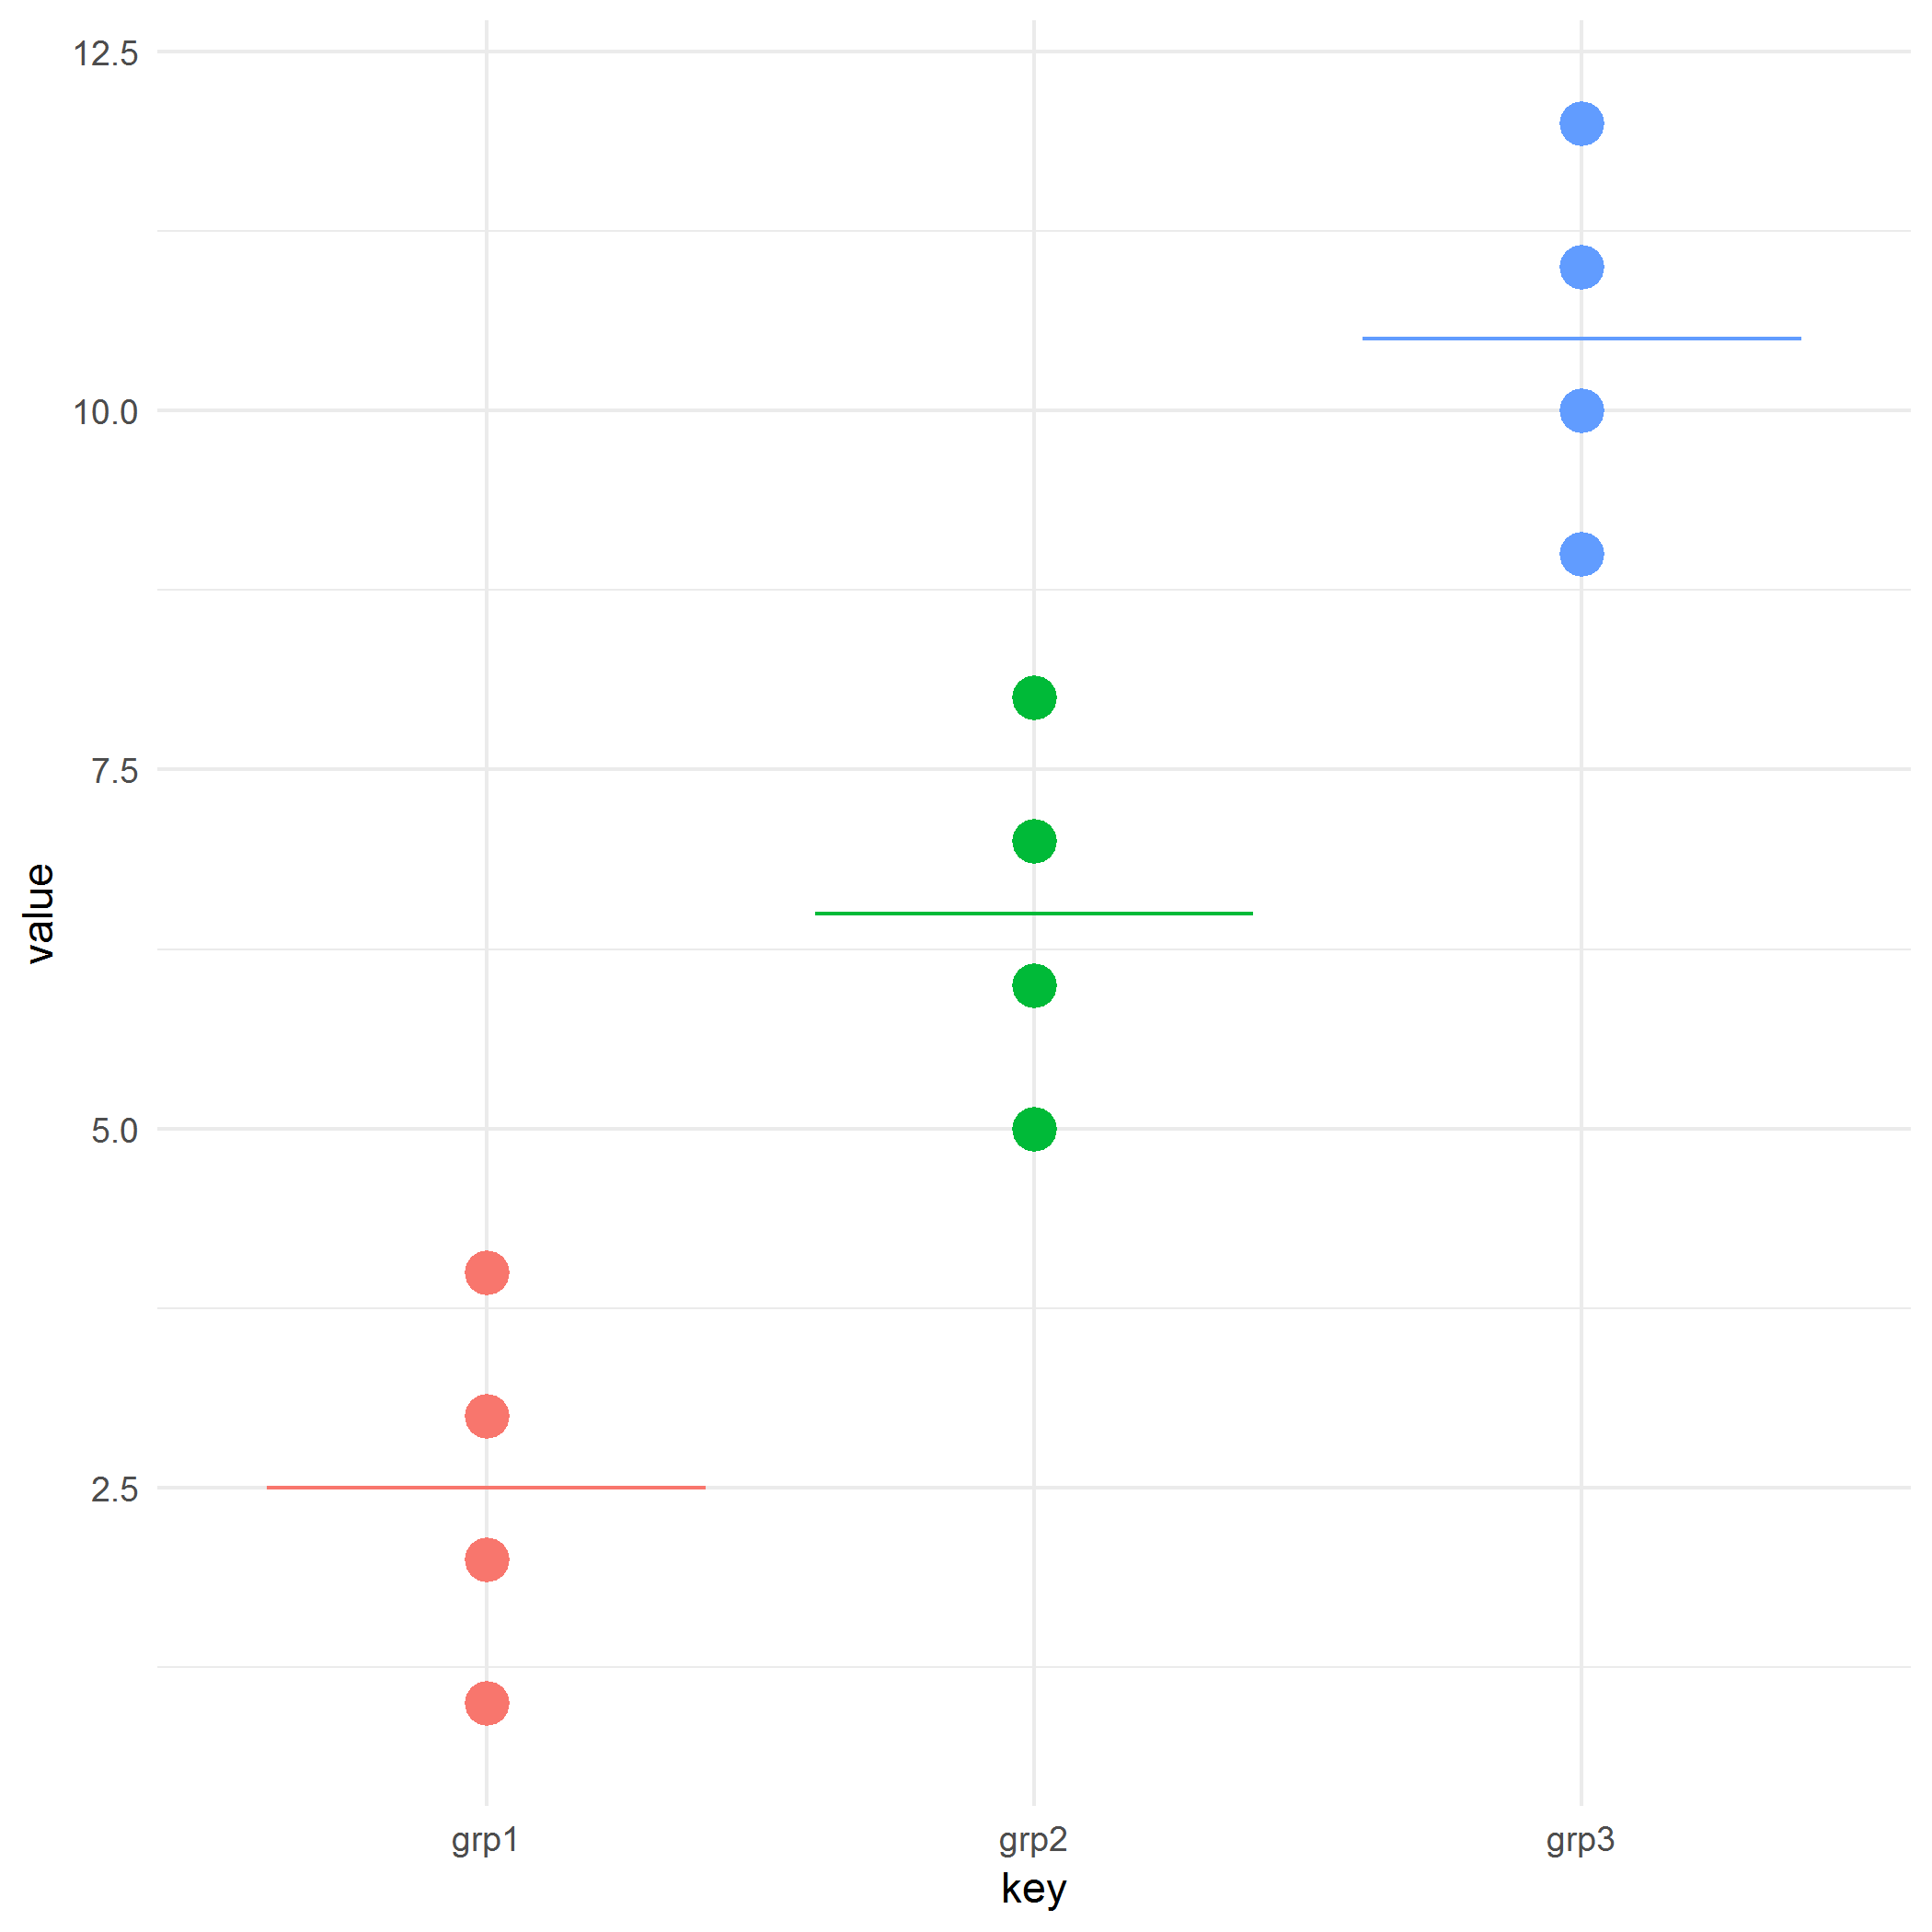
\includegraphics[width=0.6\linewidth]{cm053_files/figure-latex/unnamed-chunk-7-1}

\begin{center}\rule{0.5\linewidth}{\linethickness}\end{center}

\hypertarget{contrasts}{%
\subsection{Contrasts!}\label{contrasts}}

\begin{longtable}[]{@{}ccccc@{}}
\toprule
Contrast & Spiderman & Superman & Hulk & TNMT\tabularnewline
\midrule
\endhead
Spiderman vs.~Superman & 1 & -1 & 0 & 0\tabularnewline
Spiderman vs.~Hulk & 1 & 0 & -1 & 0\tabularnewline
Hulk vs.~TNMT & 0 & 0 & 1 & -1\tabularnewline
\bottomrule
\end{longtable}

These say: \[+1\mu_{spiderman}-1\mu_{superman}+0\mu_{hulk}+0\mu_{TNMT}\]
\[+1\mu_{spiderman}+0\mu_{superman}-1\mu_{hulk}+0\mu_{TNMT}\]
\[0\mu_{spiderman}+0\mu_{superman}+1\mu_{hulk}-1\mu_{TNMT}\]

\begin{center}\rule{0.5\linewidth}{\linethickness}\end{center}

\hypertarget{contrasts-1}{%
\subsection{Contrasts!}\label{contrasts-1}}

\[+1\mu_{spiderman}-1\mu_{superman}+0\mu_{hulk}+0\mu_{TNMT}\rightarrow\mu_{spiderman}-\mu_{superman}=0\]
\[+1\mu_{spiderman}+0\mu_{superman}-1\mu_{hulk}+0\mu_{TNMT}\rightarrow\mu_{spiderman}-\mu_{hulk}=0\]
\[0\mu_{spiderman}+0\mu_{superman}+1\mu_{hulk}-1\mu_{TNMT}\rightarrow\mu_{hulk}-\mu_{TNMT}=0\]

\begin{center}\rule{0.5\linewidth}{\linethickness}\end{center}

\hypertarget{doing-all-pairwise-contrasts-in-r}{%
\subsection{Doing all pairwise contrasts in
R}\label{doing-all-pairwise-contrasts-in-r}}

\begin{Shaded}
\begin{Highlighting}[]
\KeywordTok{pairwise.t.test}\NormalTok{(superhero}\OperatorTok{$}\NormalTok{injury,superhero}\OperatorTok{$}\NormalTok{hero,}\DataTypeTok{p.adjust.method=}\StringTok{"none"}\NormalTok{)}
\end{Highlighting}
\end{Shaded}

\begin{verbatim}

    Pairwise comparisons using t tests with pooled SD 

data:  superhero$injury and superhero$hero 

         Spiderman Superman Hulk   
Superman 0.02222   -        -      
Hulk     0.26156   0.00165  -      
TMNT     0.12144   0.00056  0.64897

P value adjustment method: none 
\end{verbatim}

\begin{quote}
Base R's output=just the \emph{p}'s, please!
\end{quote}

\begin{center}\rule{0.5\linewidth}{\linethickness}\end{center}

\hypertarget{doing-all-pairwise-contrasts-in-r-better}{%
\subsection{Doing all pairwise contrasts in R
(better)}\label{doing-all-pairwise-contrasts-in-r-better}}

\begin{Shaded}
\begin{Highlighting}[]
\KeywordTok{library}\NormalTok{(multcomp)}
\NormalTok{mcp <-}\StringTok{ }\KeywordTok{glht}\NormalTok{(heroaov,}\DataTypeTok{linfct=}\KeywordTok{mcp}\NormalTok{(}\DataTypeTok{hero=}\StringTok{"Tukey"}\NormalTok{)) }\CommentTok{# "Tukey" sets up the pairwise comparisons (computes the estimate and SE, but not the correction. see "test" below) }
\CommentTok{#summary(mcp) # Tukeys with single-step adjusted p-value}
\CommentTok{#summary(mcp, test=univariate()) #like a set of paired-ts (pooled sd 2 groups), but with pooled sd from all groups) - same as pairwise.t.test() above}
\KeywordTok{summary}\NormalTok{(mcp,}\DataTypeTok{test=}\KeywordTok{adjusted}\NormalTok{(}\StringTok{"none"}\NormalTok{)) }\CommentTok{#Same as pairwise.t.test() above }
\end{Highlighting}
\end{Shaded}

You get:

\begin{itemize}
\tightlist
\item
  the \emph{p}'s \textbf{plus}
\item
  the \emph{t}'s
\item
  the \(\psi\)'s
\item
  the \(SE_{\psi}\)'s
\item
  oh my!
\end{itemize}

\begin{center}\rule{0.5\linewidth}{\linethickness}\end{center}

\hypertarget{doing-all-pairwise-contrasts-in-r-better-1}{%
\subsection{Doing all pairwise contrasts in R
(better)}\label{doing-all-pairwise-contrasts-in-r-better-1}}

\begin{verbatim}

     Simultaneous Tests for General Linear Hypotheses

Multiple Comparisons of Means: Tukey Contrasts


Fit: aov(formula = injury ~ hero, data = superhero)

Linear Hypotheses:
                          Estimate Std. Error t value Pr(>|t|)    
Superman - Spiderman == 0   19.667      7.934   2.479 0.022218 *  
Hulk - Spiderman == 0       -9.167      7.934  -1.155 0.261564    
TMNT - Spiderman == 0      -12.833      7.934  -1.617 0.121436    
Hulk - Superman == 0       -28.833      7.934  -3.634 0.001652 ** 
TMNT - Superman == 0       -32.500      7.934  -4.096 0.000562 ***
TMNT - Hulk == 0            -3.667      7.934  -0.462 0.648969    
---
Signif. codes:  0 '***' 0.001 '**' 0.01 '*' 0.05 '.' 0.1 ' ' 1
(Adjusted p values reported -- none method)
\end{verbatim}

\begin{center}\rule{0.5\linewidth}{\linethickness}\end{center}

\hypertarget{where-are-these-numbers-coming-from}{%
\subsection{Where are these numbers coming
from?}\label{where-are-these-numbers-coming-from}}

\[estimate=\psi=\frac{\sum_{j=1}^kc_j\bar{y_j}}{\hat{\sigma_{\psi}}}\]

where\ldots{}
\[SE_{est}=\hat{\sigma_{\psi}}=\sqrt{MS_{error}\times{(\frac{1}{n_1}+\frac{1}{n_2})}}\]

And the \emph{c} terms are contrast coefficients. Thus a more general
formula is:

\[t_{contrast}=\frac{estimate}{SE_{est}}=\frac{\psi}{\hat{\sigma_{\psi}}}=\frac{\sum_{j=1}^kc_j\bar{y_j}}{\sqrt{MS_{error}\times{\frac{\sum_{j=1}^kc_j^2}{n_j}}}}\]

\begin{center}\rule{0.5\linewidth}{\linethickness}\end{center}

\hypertarget{this-is-different-from-the-independent-samples-t-test}{%
\subsection{\texorpdfstring{This is different from the independent
samples \emph{t}
test}{This is different from the independent samples t test}}\label{this-is-different-from-the-independent-samples-t-test}}

\[t=\frac{(\bar{y}_1-\bar{y}_2)-(\mu_1-\mu_2)}{\sqrt{\frac{(n_1-1)s_{y_1}^2+(n_2-1)s_{y_2}^2}{n_1+n_2-2}}}\]

Which is usually just written as:
\[t=\frac{(\bar{y}_1-\bar{y}_2)}{\sqrt{\frac{(n_1-1)s_{y_1}^2+(n_2-1)s_{y_2}^2}{n_1+n_2-2}}}\]

\begin{center}\rule{0.5\linewidth}{\linethickness}\end{center}

\hypertarget{defining-contrast-coefficients}{%
\subsection{Defining contrast
coefficients}\label{defining-contrast-coefficients}}

We base the \emph{c} terms off of your hypotheses. Let's take a look at
the superhero data:

\begin{verbatim}
# A tibble: 4 x 4
  hero       mean    sd     n
  <fct>     <dbl> <dbl> <int>
1 Spiderman  40.7 14.0      6
2 Superman   60.3 17.9      6
3 Hulk       31.5 12.8      6
4 TMNT       27.8  8.73     6
\end{verbatim}

\begin{center}\rule{0.5\linewidth}{\linethickness}\end{center}

\hypertarget{defining-contrast-coefficients-contrast-1}{%
\subsection{Defining contrast coefficients: contrast
1}\label{defining-contrast-coefficients-contrast-1}}

\begin{longtable}[]{@{}ccccc@{}}
\toprule
Contrast & Spiderman & Superman & Hulk & TNMT\tabularnewline
\midrule
\endhead
Spiderman vs.~Superman & 1 & -1 & 0 & 0\tabularnewline
\(\bar{y_j}\) & 40.67 & 60.33 & 31.5 & 27.83\tabularnewline
\bottomrule
\end{longtable}

\[\psi=\sum_{j=1}^kc_j\bar{y_j}=(1)\times{40.67}+(-1)\times{60.33}=-19.667\]

\[\hat{\sigma_{\psi}}=\sqrt{188.85\times{(\frac{1}{6}+\frac{1}{6})}}=\sqrt{188.85\times{.333}}=7.934\]

\[t_{contrast}=\frac{\psi}{\hat{\sigma_{\psi}}}=\frac{-19.667}{7.934}=-2.479\]

\begin{Shaded}
\begin{Highlighting}[]
\DecValTok{2}\OperatorTok{*}\NormalTok{(}\DecValTok{1}\OperatorTok{-}\KeywordTok{pt}\NormalTok{(}\FloatTok{2.479}\NormalTok{,}\DecValTok{20}\NormalTok{)) }\CommentTok{#unadjusted 2-tailed p-value; note the df!}
\end{Highlighting}
\end{Shaded}

\begin{verbatim}
[1] 0.02220591
\end{verbatim}

\begin{center}\rule{0.5\linewidth}{\linethickness}\end{center}

\hypertarget{contrast-degrees-of-freedom}{%
\subsection{Contrast degrees of
freedom}\label{contrast-degrees-of-freedom}}

For the pairwise \emph{t} tests ( \(t_{contrast}\) ), the degrees of
freedom for \textbf{each} contrast are the same: \emph{N-k} (where
\emph{N}= total participants and \emph{k}=number of groups)

If we were to conduct an independent samples \emph{t} test, what would
the degrees of freedom be? * The answer is: \(n_1+n_2-2\) * This is the
same as \emph{N-k}, where \emph{k} must always be 2 for the independent
samples \emph{t}-test. * In our example contrast, this is the difference
between 20 and 10 degrees of freedom

\begin{center}\rule{0.5\linewidth}{\linethickness}\end{center}

\hypertarget{increased-degrees-of-freedom}{%
\subsection{Increased degrees of
freedom}\label{increased-degrees-of-freedom}}

\begin{longtable}[]{@{}cc@{}}
\toprule
Degrees of Freedom & \(\alpha=.05,\:2-tailed\)\tabularnewline
\midrule
\endhead
10 & \textbf{2.228}\tabularnewline
11 & 2.201\tabularnewline
12 & 2.179\tabularnewline
13 & 2.160\tabularnewline
14 & 2.145\tabularnewline
15 & 2.131\tabularnewline
16 & 2.120\tabularnewline
17 & 2.110\tabularnewline
18 & 2.101\tabularnewline
19 & 2.093\tabularnewline
20 & \textbf{2.086}\tabularnewline
\bottomrule
\end{longtable}

\begin{center}\rule{0.5\linewidth}{\linethickness}\end{center}

\hypertarget{another-post-hoc-option}{%
\subsection{Another post-hoc option}\label{another-post-hoc-option}}

The Tukey Honestly Significant Difference (HSD) is a single-step
procedure that analyzes all possible pairwise contrasts between group
means.

Instead of a \emph{t} statistic ( \(t_{contrast}\) ), now we have: * The
HSD value for a family of contrasts * The Tukey statistic,
\(q_{contrast}\), for each individual contrast within the family * Both
will lead you to the same conclusion

\begin{center}\rule{0.5\linewidth}{\linethickness}\end{center}

\hypertarget{tukey-honestly-significant-difference-hsd}{%
\subsection{Tukey Honestly Significant Difference
(HSD)}\label{tukey-honestly-significant-difference-hsd}}

\[HSD=q_{tukey}\sqrt{\frac{MSE}{2}({\frac{1}{n_1}+\frac{1}{n_2}})}\]

\begin{Shaded}
\begin{Highlighting}[]
\NormalTok{mse <-}\StringTok{ }\FloatTok{188.85}
\NormalTok{ngroups <-}\StringTok{ }\DecValTok{4} \CommentTok{#4 groups, so 4 means}
\NormalTok{dfmse <-}\StringTok{ }\DecValTok{20} \CommentTok{#see ANOVA source table}
\NormalTok{q_tuk <-}\StringTok{ }\KeywordTok{qtukey}\NormalTok{(.}\DecValTok{95}\NormalTok{,ngroups,dfmse)}
\NormalTok{q_tuk}
\end{Highlighting}
\end{Shaded}

\begin{verbatim}
[1] 3.958293
\end{verbatim}

\[HSD=3.958\times\sqrt{\frac{188.85}{2}({\frac{1}{6}+\frac{1}{6}})}=22.36\]

So, any mean difference larger than 22.36 we will consider significant
according to Tukey HSD.

\begin{center}\rule{0.5\linewidth}{\linethickness}\end{center}

\hypertarget{which-differences-are-than-our-hsd-of-22.36}{%
\subsection{Which differences are \textgreater{} than our HSD of
22.36?}\label{which-differences-are-than-our-hsd-of-22.36}}

\begin{verbatim}

     Simultaneous Tests for General Linear Hypotheses

Multiple Comparisons of Means: Tukey Contrasts


Fit: aov(formula = injury ~ hero, data = superhero)

Linear Hypotheses:
                          Estimate Std. Error t value Pr(>|t|)   
Superman - Spiderman == 0   19.667      7.934   2.479  0.09446 . 
Hulk - Spiderman == 0       -9.167      7.934  -1.155  0.66072   
TMNT - Spiderman == 0      -12.833      7.934  -1.617  0.39163   
Hulk - Superman == 0       -28.833      7.934  -3.634  0.00856 **
TMNT - Superman == 0       -32.500      7.934  -4.096  0.00293 **
TMNT - Hulk == 0            -3.667      7.934  -0.462  0.96643   
---
Signif. codes:  0 '***' 0.001 '**' 0.01 '*' 0.05 '.' 0.1 ' ' 1
(Adjusted p values reported -- single-step method)
\end{verbatim}

\begin{center}\rule{0.5\linewidth}{\linethickness}\end{center}

\hypertarget{but-wait}{%
\subsection{But wait!}\label{but-wait}}

\hypertarget{those-p-values-are-different-than-before}{%
\subsubsection{\texorpdfstring{Those \emph{p}-values are different than
before!}{Those p-values are different than before!}}\label{those-p-values-are-different-than-before}}

Old \(p\)'s\ldots{}

\begin{verbatim}
Superman - Spiderman     Hulk - Spiderman     TMNT - Spiderman 
        0.0222176879         0.2615640877         0.1214364334 
     Hulk - Superman      TMNT - Superman          TMNT - Hulk 
        0.0016520896         0.0005617408         0.6489687464 
\end{verbatim}

New \(p\)'s\ldots{}

\begin{verbatim}
Superman - Spiderman     Hulk - Spiderman     TMNT - Spiderman 
         0.094345515          0.660718016          0.391779399 
     Hulk - Superman      TMNT - Superman          TMNT - Hulk 
         0.008110220          0.002766473          0.966423491 
\end{verbatim}

\begin{center}\rule{0.5\linewidth}{\linethickness}\end{center}

\hypertarget{tukey-hsd}{%
\subsection{Tukey HSD}\label{tukey-hsd}}

That's because the \emph{p} value is based on a \textbf{new} statistic (
\(q_{contrast}\) ), but only the \emph{p} values in the table
\emph{glht} provides changed (which is confusing!). Let's see that new
statistic\ldots{}

For any specific contrast we can calculate:
\[q_{contrast}=\frac{|\psi|}{\sqrt{\frac{MSE}{2}({\frac{1}{n_1}+\frac{1}{n_2}})}}\]

\begin{Shaded}
\begin{Highlighting}[]
\NormalTok{psi <-}\StringTok{ }\KeywordTok{abs}\NormalTok{(}\OperatorTok{-}\FloatTok{19.667}\NormalTok{) }
\NormalTok{se <-}\StringTok{ }\KeywordTok{sqrt}\NormalTok{((mse}\OperatorTok{/}\DecValTok{2}\NormalTok{)}\OperatorTok{*}\NormalTok{(}\DecValTok{1}\OperatorTok{/}\DecValTok{6}\OperatorTok{+}\DecValTok{1}\OperatorTok{/}\DecValTok{6}\NormalTok{))}
\NormalTok{qobs <-}\StringTok{ }\NormalTok{psi}\OperatorTok{/}\NormalTok{se}
\NormalTok{se}
\end{Highlighting}
\end{Shaded}

\begin{verbatim}
[1] 5.610258
\end{verbatim}

\begin{Shaded}
\begin{Highlighting}[]
\NormalTok{qobs}
\end{Highlighting}
\end{Shaded}

\begin{verbatim}
[1] 3.505543
\end{verbatim}

\[q_{contrast}=\frac{19.667}{\sqrt{\frac{188.85}{2}({\frac{1}{6}+\frac{1}{6}})}}=3.506\]

\begin{center}\rule{0.5\linewidth}{\linethickness}\end{center}

\hypertarget{finding-the-p-value-for-tukey-hsd}{%
\subsection{\texorpdfstring{Finding the \emph{p}-value for Tukey
HSD}{Finding the p-value for Tukey HSD}}\label{finding-the-p-value-for-tukey-hsd}}

So, according to Tukey HSD, we have the following:
\[q_{Spiderman\:v.\:Superman}=3.506\]

Because our critical \(q_{tukey}\) was 3.958, we know that our
\(q_{contrast}\) of 3.506 is not significant. In fact, the
\emph{p}-value for our \(q_{contrast}\) is\ldots{}

\begin{Shaded}
\begin{Highlighting}[]
\KeywordTok{ptukey}\NormalTok{(qobs,ngroups,dfmse,}\DataTypeTok{lower.tail=}\NormalTok{F)}
\end{Highlighting}
\end{Shaded}

\begin{verbatim}
[1] 0.09425035
\end{verbatim}

\begin{itemize}
\tightlist
\item
  \textbf{N.B.} \#1: This is the same \emph{p} value in the \emph{glht}
  output.
\item
  \textbf{N.B.} \#2: We reach the same conclusion based on comparing our
  difference in means to the HSD: for Spiderman vs.~Superman, 19.667
  \textless{} 22.36.
\end{itemize}

\begin{center}\rule{0.5\linewidth}{\linethickness}\end{center}

\hypertarget{note-about-tukey-hsd-in-glht}{%
\subsection{\texorpdfstring{Note about Tukey HSD in
\emph{glht}}{Note about Tukey HSD in glht}}\label{note-about-tukey-hsd-in-glht}}

We have just observed something important in the \emph{glht} output.

\begin{itemize}
\tightlist
\item
  The \emph{t} statistics correspond to our pairwise \emph{t} test (
  \(t_{contrast}\) ). This is a standard \emph{t} distributed variable.
\item
  The \emph{p}-values correspond to the Tukey Studentized Range
  Distribution ( \(q_{contrast}\) ).
\end{itemize}

So in our example contrast between Spiderman and Superman:

\begin{longtable}[]{@{}ccccc@{}}
\toprule
Distribution of Statistic & Statistic & SE & \emph{p}-value &
tails\tabularnewline
\midrule
\endhead
Student \emph{t} Distribution & 2.479 & 7.93 & .022 & 2 (can be
1)\tabularnewline
Tukey Studentized Range Distribution & 3.506 & 5.61 & .094 & always
1\tabularnewline
\bottomrule
\end{longtable}

\begin{center}\rule{0.5\linewidth}{\linethickness}\end{center}

\hypertarget{to-sum-up}{%
\subsection{To sum up\ldots{}}\label{to-sum-up}}

\hypertarget{those-p-values-are-different-than-before-yes-they-are.}{%
\subsubsection{\texorpdfstring{Those \emph{p}-values are different than
before! Yes they
are.}{Those p-values are different than before! Yes they are.}}\label{those-p-values-are-different-than-before-yes-they-are.}}

Old \(p\)'s based on Student \emph{t} distributed statistic (
\(t_{contrast}\) )\ldots{}

\begin{verbatim}
Superman - Spiderman     Hulk - Spiderman     TMNT - Spiderman 
        0.0222176879         0.2615640877         0.1214364334 
     Hulk - Superman      TMNT - Superman          TMNT - Hulk 
        0.0016520896         0.0005617408         0.6489687464 
\end{verbatim}

New \(p\)'s based on Tukey Studentized Range statistic (
\(q_{contrast}\) )\ldots{}

\begin{verbatim}
Superman - Spiderman     Hulk - Spiderman     TMNT - Spiderman 
         0.094393256          0.660746731          0.391763753 
     Hulk - Superman      TMNT - Superman          TMNT - Hulk 
         0.008277121          0.002834529          0.966428841 
\end{verbatim}

\begin{center}\rule{0.5\linewidth}{\linethickness}\end{center}

\hypertarget{why-not-just-do-a-bunch-of-t-tests}{%
\subsection{\texorpdfstring{Why not just do a bunch of
\emph{t}-tests?}{Why not just do a bunch of t-tests?}}\label{why-not-just-do-a-bunch-of-t-tests}}

\begin{itemize}
\item
  First, note that pairwise contrasts use the degrees of freedom
  \textbf{based on all groups in your sample}, rather than for just the
  two groups in the contrast. This increases your statistical power!
\item
  Second, pairwise contrasts (whether \(t_{contrast}\) or
  \(q_{contrast}\) ) base the standard error estimate (i.e., the
  denominator) on the weighted mean square error ( \(MS_{error}\) ) from
  the overall ANOVA. Again, this tends to increase power!
\item
  But, each individual pairwise contrast is designed to control the
  probability of false rejection at \(\alpha\). Unfortunately, if our
  data analysis involves many hypothesis tests (and thus many
  contrasts), the probability of at least one Type I error increases
  rather sharply with the number of contrasts.
\end{itemize}

\begin{center}\rule{0.5\linewidth}{\linethickness}\end{center}

\hypertarget{probabilityat-least-one-error}{%
\subsection{Probability(at least one
error)}\label{probabilityat-least-one-error}}

For example: * If there are \emph{m} tests * They are independent * Each
is performed with \(\alpha\)=.05 * All alternative hypotheses are
\textbf{true} * What is the probability of at least one Type I error?

\begin{center}\rule{0.5\linewidth}{\linethickness}\end{center}

\hypertarget{probability-refresher}{%
\subsection{Probability refresher}\label{probability-refresher}}

If we have 3 levels of a factor, and want to compare all three to each
other: 1. Contrast 1 vs.~2 ( \(\alpha=.05\) ) 2. Contrast 2 vs.~3 (
\(\alpha=.05\) ) 3. Contrast 1 vs.~3 ( \(\alpha=.05\) )

Probabilities:

\begin{itemize}
\item
  What is the probability that I will \textbf{incorrectly reject} all
  three null hypotheses?
  \[P(\alpha)\times{P(\alpha)}\times{P(\alpha)}=(.05)(.05)(.05)=.000125\]
\item
  Using the same logic, what is the probability that I will
  \textbf{correctly reject} all three null hypotheses?
  \[P(1-\alpha)\times{P(1-\alpha)}\times{P(1-\alpha)}=(.95)(.95)(.95)=.8574\]
\item
  Hmmm\ldots{}
\end{itemize}

\begin{center}\rule{0.5\linewidth}{\linethickness}\end{center}

\hypertarget{probabilityat-least-one-error-1}{%
\subsection{Probability(at least one
error)}\label{probabilityat-least-one-error-1}}

\[P(Type \: I \: error)=\alpha\]
\[P(no \: Type \: I \: error)=1-\alpha\]
\[P(no \:Type\:I\:errors\:in\:m\:tests)=(1-\alpha)^m\]
\[P(at\:least\:one\:Type\:I\:errors\:in\:m\:tests)=1-(1-\alpha)^m\]

\begin{center}\rule{0.5\linewidth}{\linethickness}\end{center}

\hypertarget{family-wise-error-rate-fwer}{%
\subsection{Family-wise error rate
(FWER)}\label{family-wise-error-rate-fwer}}

The probability that I make \textbf{zero} errors:
\[P(1-\alpha)\times{P(1-\alpha)}\times{P(1-\alpha)}=(.95)(.95)(.95)=.8574\]
The \emph{family-wise error rate}:
\[P(at\:least\:one\:error)=1-P(no\:errors)=1-.8574=.1426 > .05\] Thus,
the probability that I will make at least one Type I error is
\textgreater{} .05

\[\alpha_{family}>\alpha_{per\:test}\]

\begin{center}\rule{0.5\linewidth}{\linethickness}\end{center}

\hypertarget{we-can-plot-this}{%
\subsection{We can plot this\ldots{}}\label{we-can-plot-this}}

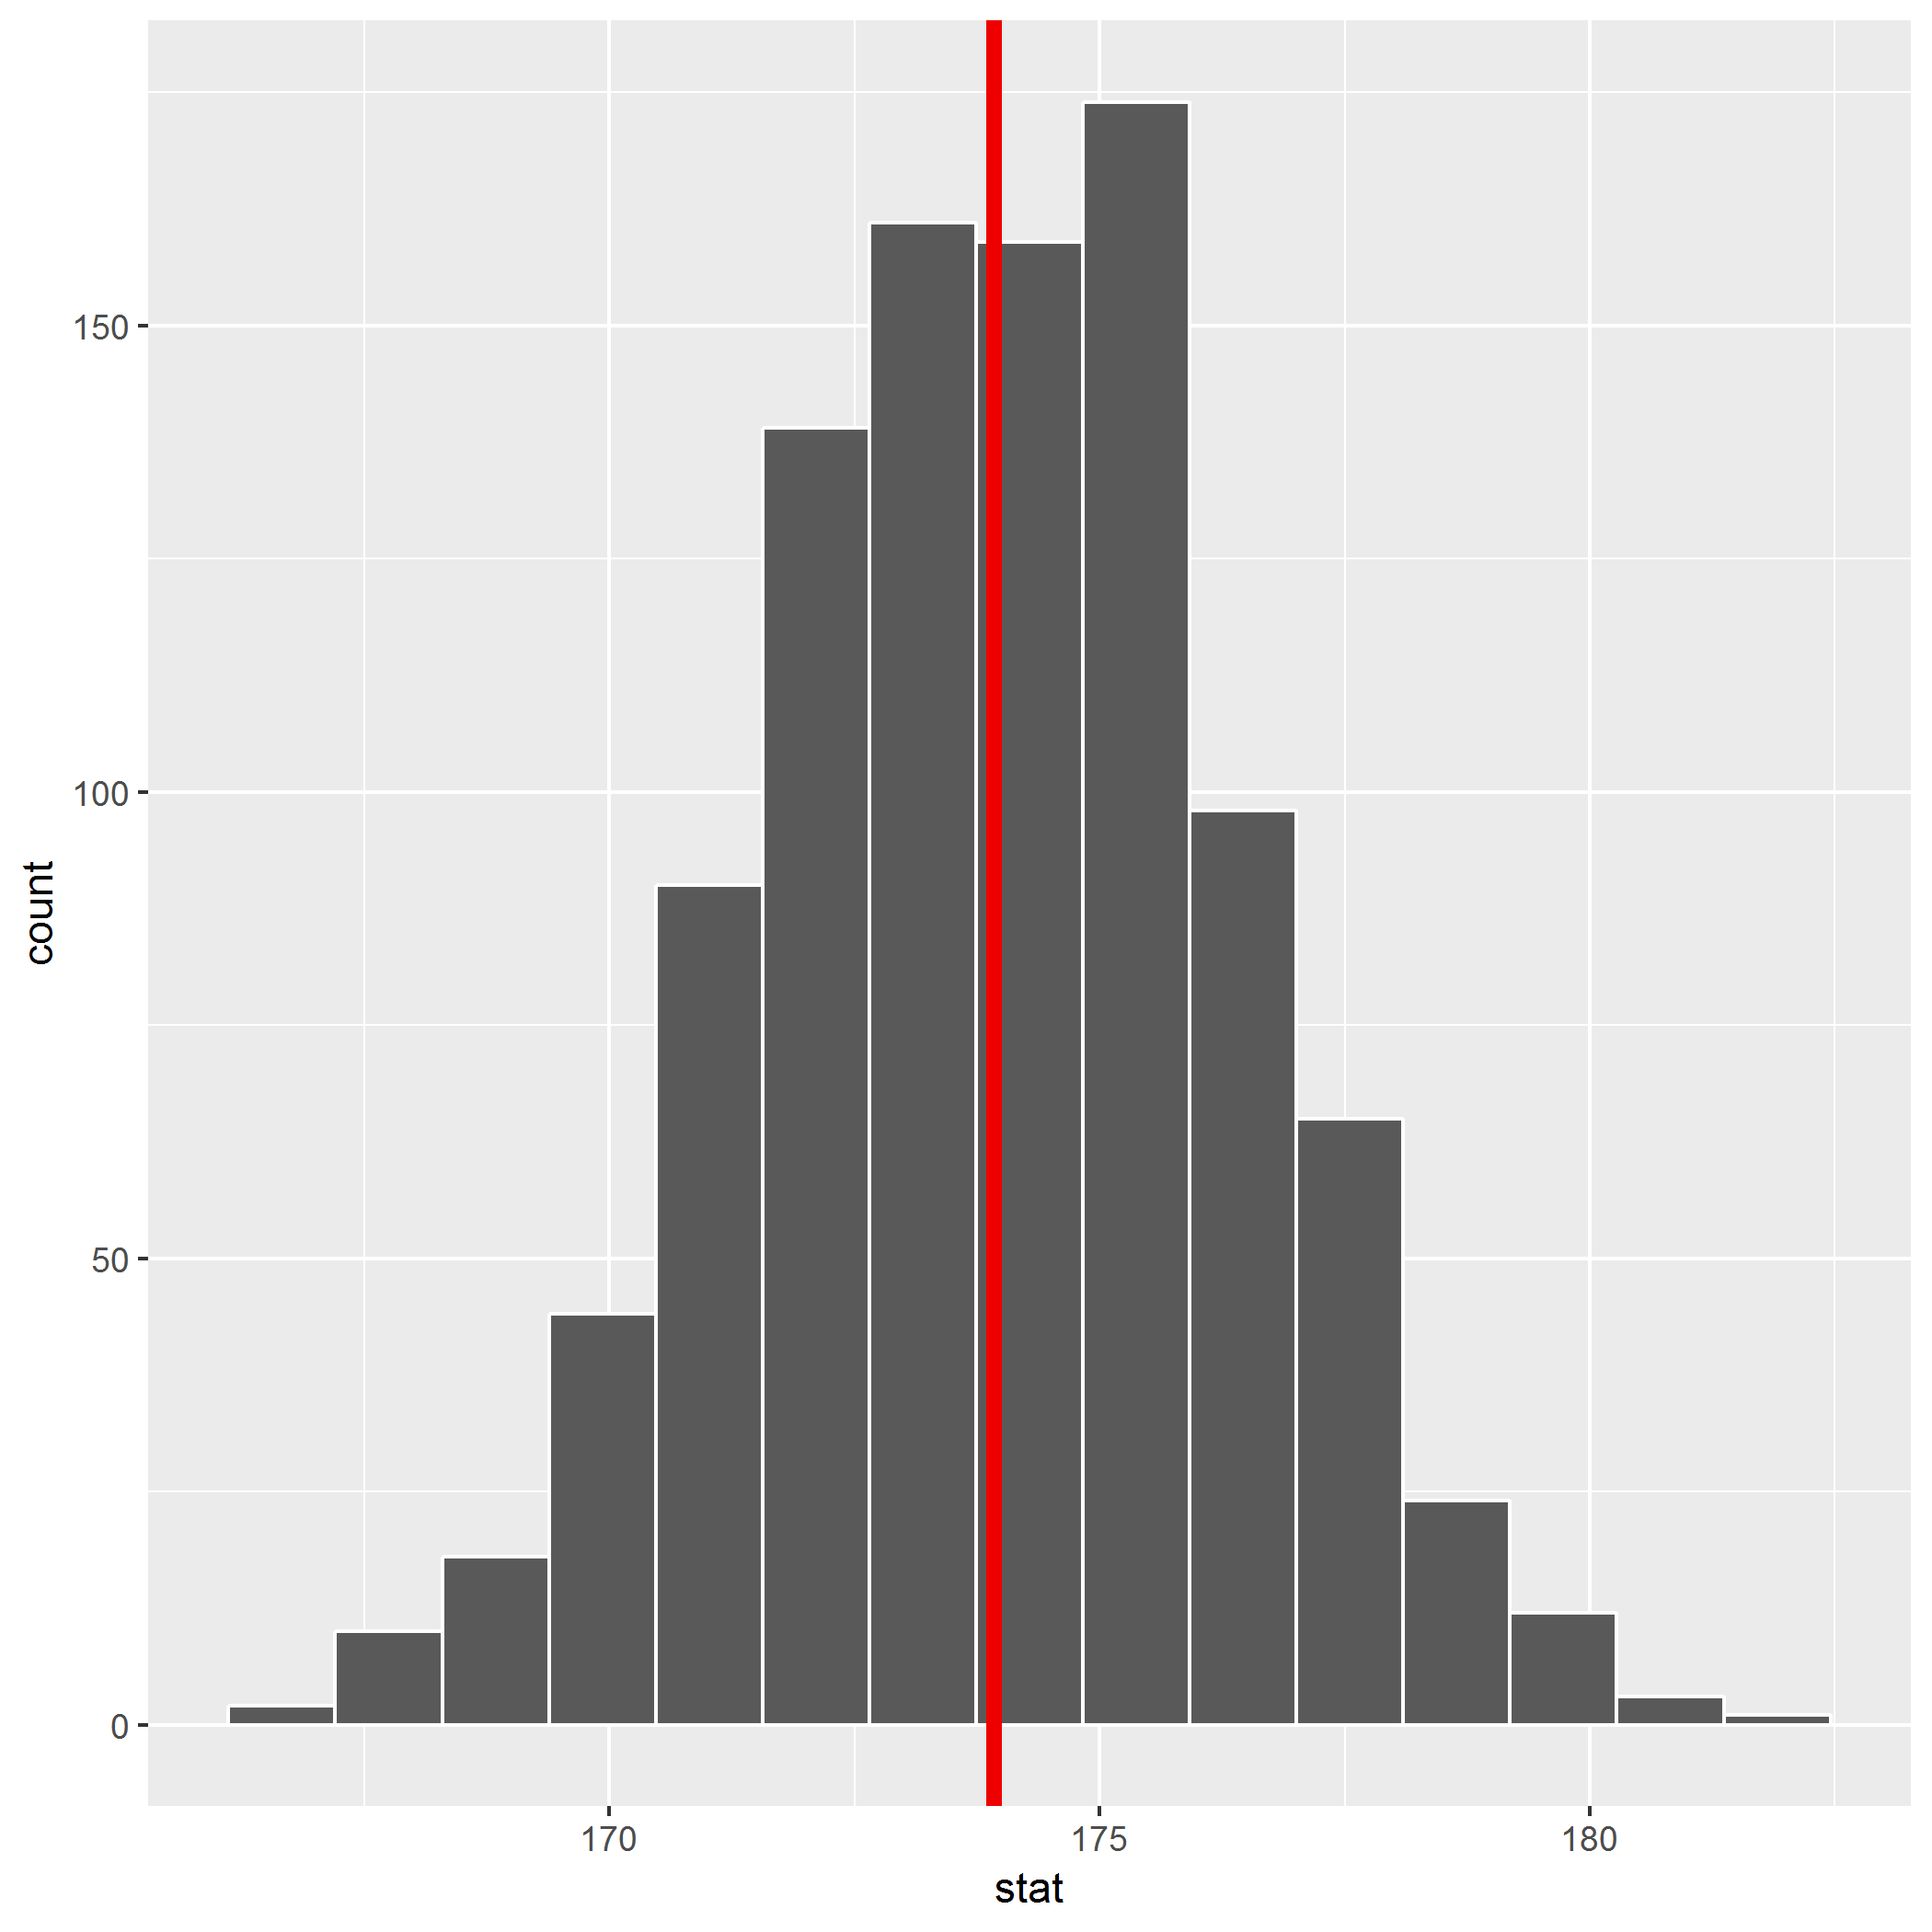
\includegraphics[width=0.6\linewidth]{cm053_files/figure-latex/unnamed-chunk-23-1}

\hypertarget{doing-all-pairwise-contrasts-in-r-better-2}{%
\subsection{Doing all pairwise contrasts in R
better*}\label{doing-all-pairwise-contrasts-in-r-better-2}}

\begin{Shaded}
\begin{Highlighting}[]
\KeywordTok{summary}\NormalTok{(mcp, }\DataTypeTok{test =} \KeywordTok{adjusted}\NormalTok{(}\StringTok{"BH"}\NormalTok{)) }\CommentTok{#Tukey HSD + BH p-adjustment!}
\end{Highlighting}
\end{Shaded}

\begin{verbatim}

     Simultaneous Tests for General Linear Hypotheses

Multiple Comparisons of Means: Tukey Contrasts


Fit: aov(formula = injury ~ hero, data = superhero)

Linear Hypotheses:
                          Estimate Std. Error t value Pr(>|t|)   
Superman - Spiderman == 0   19.667      7.934   2.479  0.04444 * 
Hulk - Spiderman == 0       -9.167      7.934  -1.155  0.31388   
TMNT - Spiderman == 0      -12.833      7.934  -1.617  0.18215   
Hulk - Superman == 0       -28.833      7.934  -3.634  0.00496 **
TMNT - Superman == 0       -32.500      7.934  -4.096  0.00337 **
TMNT - Hulk == 0            -3.667      7.934  -0.462  0.64897   
---
Signif. codes:  0 '***' 0.001 '**' 0.01 '*' 0.05 '.' 0.1 ' ' 1
(Adjusted p values reported -- BH method)
\end{verbatim}

\begin{center}\rule{0.5\linewidth}{\linethickness}\end{center}

\hypertarget{but-wait-1}{%
\subsection{But wait!}\label{but-wait-1}}

\hypertarget{you-changed-the-p-values-again-yes-i-did.}{%
\subsubsection{\texorpdfstring{You changed the \emph{p}-values again!
Yes I
did.}{You changed the p-values again! Yes I did.}}\label{you-changed-the-p-values-again-yes-i-did.}}

Unadjusted \(p\)'s based on Tukey's HSD\ldots{}

\begin{verbatim}
Superman - Spiderman     Hulk - Spiderman     TMNT - Spiderman 
         0.094393256          0.660746731          0.391763753 
     Hulk - Superman      TMNT - Superman          TMNT - Hulk 
         0.008277121          0.002834529          0.966428841 
\end{verbatim}

Tukey HSD \(p\)'s with Benjamini-Hochberg adjustment\ldots{}

\begin{verbatim}
Superman - Spiderman     Hulk - Spiderman     TMNT - Spiderman 
         0.044435376          0.313876905          0.182154650 
     Hulk - Superman      TMNT - Superman          TMNT - Hulk 
         0.004956269          0.003370445          0.648968746 
\end{verbatim}

\begin{center}\rule{0.5\linewidth}{\linethickness}\end{center}

\hypertarget{the-benjamini-hochberg-false-discovery-rate-fdr}{%
\subsection{The Benjamini-Hochberg False Discovery Rate
(FDR)}\label{the-benjamini-hochberg-false-discovery-rate-fdr}}

The basic idea of the FDR is to try to achieve the smallest possible
fraction of false signals among all those that appear to be true (i.e.,
significant).

Said another way: we estimate the expected proportion of false
rejections among all rejected null hypotheses and attempt to keep it
under a threshold level.

Using the FDR method, we are trying to control the number of ``false
discoveries'' rather than the number of ``false positives.''

\begin{quote}
What is the difference?
\end{quote}

\begin{center}\rule{0.5\linewidth}{\linethickness}\end{center}

\hypertarget{false-positives-false-discoveries}{%
\subsection{False Positives \& False
Discoveries}\label{false-positives-false-discoveries}}

Let's revisit the good ol' decision table. Let \emph{m} be the total
number of hypotheses tested.

\begin{longtable}[]{@{}cccc@{}}
\toprule
& Decision: Do not reject \(H_0\) & Decision: Reject \(H_0\) &
Total\tabularnewline
\midrule
\endhead
\(H_0\) is true & U \emph{True Negative} & V \textbf{Type I
error}/\emph{False Positive} & \(m_0\)\tabularnewline
\(H_0\) is false & T \textbf{Type II error}/\emph{False Negative} & S
\emph{True Positive} & \(m-m_0\)\tabularnewline
Total & \(m-R\) & \(R\) & \(m\)\tabularnewline
\bottomrule
\end{longtable}

The false positive rate is: \[FPR=\frac{V}{m_0}\]

The false discovery rate is: \[FDR=\frac{V}{R}\]

\begin{center}\rule{0.5\linewidth}{\linethickness}\end{center}

\hypertarget{false-positives-false-discoveries-1}{%
\subsection{False Positives \& False
Discoveries}\label{false-positives-false-discoveries-1}}

The \textbf{false positive rate} is:
\[FPR=\frac{number\:of\:falsely\:rejected\:H_0s}{total\:number\:of\:true\:H_0s}\]

The \textbf{false discovery rate} is:
\[FDR=\frac{number\:of\:falsely\:rejected\:H_0s}{total\:number\:of\:rejected\:H_0s}\]

Benjamini-Hochberg proposed to keep the latter less than \(\alpha\) such
that the maximum FDR is capped at \(q<\alpha\).

\begin{center}\rule{0.5\linewidth}{\linethickness}\end{center}

\hypertarget{the-fdr-method}{%
\subsection{The FDR Method}\label{the-fdr-method}}

Sort your obtained \emph{p}-values from lowest to highest, and add the
following information:

\begin{itemize}
\tightlist
\item
  \(p\) = sorted unadjusted \emph{p}-values (these can be based on any
  statistic, here Tukey HSD)
\item
  \(j\) = variable indexing the order of that contrast in the sort (
  \(j=1,\dotsc,m\) )
\item
  \(p_{BH}^*\) = critical values for \emph{p}, based on
  Benjamini-Hochberg per contrast adjustments holding \(q<.05\) (see
  next slides)
\end{itemize}

\begin{verbatim}
     TMNT - Superman Hulk - Superman Superman - Spiderman TMNT - Spiderman
p              0.003           0.008                0.094            0.392
j              1.000           2.000                3.000            4.000
p*BH           0.008           0.017                0.025            0.033
     Hulk - Spiderman TMNT - Hulk
p               0.661       0.966
j               5.000       6.000
p*BH            0.042       0.050
\end{verbatim}

\begin{center}\rule{0.5\linewidth}{\linethickness}\end{center}

\hypertarget{the-benjamini-hochberg-false-discovery-rate}{%
\subsection{The Benjamini-Hochberg False Discovery
Rate}\label{the-benjamini-hochberg-false-discovery-rate}}

The previous table can be summarized more generally as:

\begin{longtable}[]{@{}cccccc@{}}
\toprule
\begin{minipage}[b]{0.10\columnwidth}\centering
\strut
\end{minipage} & \begin{minipage}[b]{0.13\columnwidth}\centering
smallest\strut
\end{minipage} & \begin{minipage}[b]{0.10\columnwidth}\centering
\(\rightarrow\)\strut
\end{minipage} & \begin{minipage}[b]{0.10\columnwidth}\centering
\(\rightarrow\)\strut
\end{minipage} & \begin{minipage}[b]{0.25\columnwidth}\centering
\(\rightarrow\)\strut
\end{minipage} & \begin{minipage}[b]{0.15\columnwidth}\centering
largest\strut
\end{minipage}\tabularnewline
\midrule
\endhead
\begin{minipage}[t]{0.10\columnwidth}\centering
\(p-values\)\strut
\end{minipage} & \begin{minipage}[t]{0.13\columnwidth}\centering
\(p_1\)\strut
\end{minipage} & \begin{minipage}[t]{0.10\columnwidth}\centering
\(p_2\)\strut
\end{minipage} & \begin{minipage}[t]{0.10\columnwidth}\centering
\(p_3\)\strut
\end{minipage} & \begin{minipage}[t]{0.25\columnwidth}\centering
\(\dotsc\)\strut
\end{minipage} & \begin{minipage}[t]{0.15\columnwidth}\centering
\(p_m\)\strut
\end{minipage}\tabularnewline
\begin{minipage}[t]{0.10\columnwidth}\centering
\(j\)\strut
\end{minipage} & \begin{minipage}[t]{0.13\columnwidth}\centering
1\strut
\end{minipage} & \begin{minipage}[t]{0.10\columnwidth}\centering
2\strut
\end{minipage} & \begin{minipage}[t]{0.10\columnwidth}\centering
3\strut
\end{minipage} & \begin{minipage}[t]{0.25\columnwidth}\centering
\(\dotsc\)\strut
\end{minipage} & \begin{minipage}[t]{0.15\columnwidth}\centering
\(m\)\strut
\end{minipage}\tabularnewline
\begin{minipage}[t]{0.10\columnwidth}\centering
\(p_{BH}^*\)\strut
\end{minipage} & \begin{minipage}[t]{0.13\columnwidth}\centering
\(\frac{1}{m}\times{\alpha}\)\strut
\end{minipage} & \begin{minipage}[t]{0.10\columnwidth}\centering
\(\frac{2}{m}\times{\alpha}\)\strut
\end{minipage} & \begin{minipage}[t]{0.10\columnwidth}\centering
\(\frac{3}{m}\times{\alpha}\)\strut
\end{minipage} & \begin{minipage}[t]{0.25\columnwidth}\centering
\(\dotsc\)\strut
\end{minipage} & \begin{minipage}[t]{0.15\columnwidth}\centering
\(\frac{m}{m}\times{\alpha}=\alpha\)\strut
\end{minipage}\tabularnewline
\bottomrule
\end{longtable}

Where the \(p_{BH}^*\) threshold for each individual contrast is:
\[\frac{j}{m}\times{\alpha}\]

\begin{center}\rule{0.5\linewidth}{\linethickness}\end{center}

\hypertarget{decision-time}{%
\subsection{Decision Time}\label{decision-time}}

\begin{verbatim}
         TMNT - Superman Hulk - Superman Superman - Spiderman
p                  0.003           0.008                0.094
j                      1               2                    3
p*BH               0.008           0.017                0.025
Decision       REJECT H0       REJECT H0     DO NOT REJECT H0
         TMNT - Spiderman Hulk - Spiderman      TMNT - Hulk
p                   0.392            0.661            0.966
j                       4                5                6
p*BH                0.033            0.042             0.05
Decision DO NOT REJECT H0 DO NOT REJECT H0 DO NOT REJECT H0
\end{verbatim}

\begin{center}\rule{0.5\linewidth}{\linethickness}\end{center}

\hypertarget{bonferroni-method}{%
\subsection{Bonferroni Method}\label{bonferroni-method}}

A different approach to adjusting \emph{p}-values per contrast is to
control the \textbf{false positive rate} by controlling the
\emph{family-wise error rate}= \(\alpha\) .

\textbf{The idea:} if you want to control your Type I error rate at
\(\alpha=.05\) across all \emph{m} contrasts, then simply compare your
obtained \emph{p}-value with a new \(p_{Bonferroni}^*\):
\[p_{Bonferroni}^*=\frac{\alpha}{m}\]

Where \emph{m} is the maximum total number of contrasts you'll need to
perform.

\textbf{The downside:} comes at a cost of decreasing statisical power
(increasing Type II errors) and thus being overly conservative

In our current example, we conduct \emph{m}=6 contrasts total, so our
nominal per contrast \emph{p} is:
\[p_{Bonferroni}^*=\frac{.05}{6}=.008\]

\begin{center}\rule{0.5\linewidth}{\linethickness}\end{center}

\hypertarget{false-positives}{%
\subsection{False Positives}\label{false-positives}}

Recall that the \textbf{false positive rate} is:
\[FPR=\frac{number\:of\:falsely\:rejected\:H_0s}{total\:number\:of\:true\:H_0s}\]

\begin{center}\rule{0.5\linewidth}{\linethickness}\end{center}

\hypertarget{bonferroni-vs.-benjamini-hochberg}{%
\subsection{Bonferroni
vs.~Benjamini-Hochberg}\label{bonferroni-vs.-benjamini-hochberg}}

Let's compare to the BH FDR:

\begin{longtable}[]{@{}cccccc@{}}
\toprule
\begin{minipage}[b]{0.10\columnwidth}\centering
\strut
\end{minipage} & \begin{minipage}[b]{0.13\columnwidth}\centering
smallest\strut
\end{minipage} & \begin{minipage}[b]{0.10\columnwidth}\centering
\strut
\end{minipage} & \begin{minipage}[b]{0.10\columnwidth}\centering
\strut
\end{minipage} & \begin{minipage}[b]{0.25\columnwidth}\centering
\(\rightarrow\)\strut
\end{minipage} & \begin{minipage}[b]{0.15\columnwidth}\centering
largest\strut
\end{minipage}\tabularnewline
\midrule
\endhead
\begin{minipage}[t]{0.10\columnwidth}\centering
\(p-values\)\strut
\end{minipage} & \begin{minipage}[t]{0.13\columnwidth}\centering
\(p_1\)\strut
\end{minipage} & \begin{minipage}[t]{0.10\columnwidth}\centering
\(p_2\)\strut
\end{minipage} & \begin{minipage}[t]{0.10\columnwidth}\centering
\(p_3\)\strut
\end{minipage} & \begin{minipage}[t]{0.25\columnwidth}\centering
\(\dotsc\)\strut
\end{minipage} & \begin{minipage}[t]{0.15\columnwidth}\centering
\(p_m\)\strut
\end{minipage}\tabularnewline
\begin{minipage}[t]{0.10\columnwidth}\centering
\(j\)\strut
\end{minipage} & \begin{minipage}[t]{0.13\columnwidth}\centering
1\strut
\end{minipage} & \begin{minipage}[t]{0.10\columnwidth}\centering
2\strut
\end{minipage} & \begin{minipage}[t]{0.10\columnwidth}\centering
3\strut
\end{minipage} & \begin{minipage}[t]{0.25\columnwidth}\centering
\(\dotsc\)\strut
\end{minipage} & \begin{minipage}[t]{0.15\columnwidth}\centering
\(m\)\strut
\end{minipage}\tabularnewline
\begin{minipage}[t]{0.10\columnwidth}\centering
\(p_{BH}^*\)\strut
\end{minipage} & \begin{minipage}[t]{0.13\columnwidth}\centering
\(1\times{\frac{\alpha}{m}}\)\strut
\end{minipage} & \begin{minipage}[t]{0.10\columnwidth}\centering
\(2\times{\frac{\alpha}{m}}\)\strut
\end{minipage} & \begin{minipage}[t]{0.10\columnwidth}\centering
\(3\times{\frac{\alpha}{m}}\)\strut
\end{minipage} & \begin{minipage}[t]{0.25\columnwidth}\centering
\(\dotsc\)\strut
\end{minipage} & \begin{minipage}[t]{0.15\columnwidth}\centering
\(m\times{\frac{\alpha}{m}}=\alpha\)\strut
\end{minipage}\tabularnewline
\begin{minipage}[t]{0.10\columnwidth}\centering
\(p_{Bonferroni}^*\)\strut
\end{minipage} & \begin{minipage}[t]{0.13\columnwidth}\centering
\(\frac{\alpha}{m}\)\strut
\end{minipage} & \begin{minipage}[t]{0.10\columnwidth}\centering
\(\frac{\alpha}{m}\)\strut
\end{minipage} & \begin{minipage}[t]{0.10\columnwidth}\centering
\(\frac{\alpha}{m}\)\strut
\end{minipage} & \begin{minipage}[t]{0.25\columnwidth}\centering
\(\dotsc\)\strut
\end{minipage} & \begin{minipage}[t]{0.15\columnwidth}\centering
\(\frac{\alpha}{m}\)\strut
\end{minipage}\tabularnewline
\bottomrule
\end{longtable}

\begin{quote}
So for the smallest \emph{p}-value, \(p_{BH}^*\) will always equal
\(p_{Bonferroni}^*\)
\end{quote}

\begin{center}\rule{0.5\linewidth}{\linethickness}\end{center}

\hypertarget{bonferroni-vs.-benjamini-hochberg-1}{%
\subsection{Bonferroni
vs.~Benjamini-Hochberg}\label{bonferroni-vs.-benjamini-hochberg-1}}

Would our decisions have been any different if, instead of controlling
the \emph{false discovery rate} via Benjamini-Hochberg, we controlled
the \emph{family-wise error rate} via Bonferroni?

\begin{verbatim}
                     TMNT - Superman Hulk - Superman Superman - Spiderman
p                              0.003           0.008                0.094
j                                  1               2                    3
p*BH                           0.008           0.017                0.025
Decision: BH               REJECT H0       REJECT H0     DO NOT REJECT H0
p*Bonferroni                   0.008           0.008                0.008
Decision: Bonferroni       REJECT H0       REJECT H0     DO NOT REJECT H0
                     TMNT - Spiderman Hulk - Spiderman      TMNT - Hulk
p                               0.392            0.661            0.966
j                                   4                5                6
p*BH                            0.033            0.042             0.05
Decision: BH         DO NOT REJECT H0 DO NOT REJECT H0 DO NOT REJECT H0
p*Bonferroni                    0.008            0.008            0.008
Decision: Bonferroni DO NOT REJECT H0 DO NOT REJECT H0 DO NOT REJECT H0
\end{verbatim}

\begin{center}\rule{0.5\linewidth}{\linethickness}\end{center}

\hypertarget{adjusted-p-values-options}{%
\subsection{Adjusted p-values options}\label{adjusted-p-values-options}}

We just covered two \emph{p} value adjustment options:

\begin{itemize}
\tightlist
\item
  Benjamini-Hochberg (in R, ``BH'' or ``fdr'')
\item
  Bonferroni
\item
  But there are many many more\ldots{}
\end{itemize}

From \emph{multcomp}: \textgreater{} ``Shaffer'' implements
Bonferroni-adjustments taking logical constraints into account Shaffer
{[}1986{]} and ``Westfall'' takes both logical constraints and
correlations among the z statistics into account Westfall {[}1997{]}. In
addition, all adjustment methods implemented in p.adjust can be
specified as well.

From \emph{help(p.adjust)}: \textgreater{} c(``holm'', ``hochberg'',
``hommel'', ``bonferroni'', ``BH'', ``BY'', ``fdr'', ``none'')

\begin{center}\rule{0.5\linewidth}{\linethickness}\end{center}

\hypertarget{an-example}{%
\subsection{An example:}\label{an-example}}

\begin{quote}
\begin{itemize}
\tightlist
\item
  As discussed in Benjamini and Yekutieli (2001), Needleman et al (New
  England Journal of Medicine, 300, 689--695) studied the
  neuropsychologic effects of unidentified childhood exposure to lead by
  comparing various psychological and classroom performances between two
  groups of children differing in the lead level observed in their shed
  teeth.
\end{itemize}
\end{quote}

\begin{quote}
\begin{itemize}
\tightlist
\item
  While there is no doubt that high levels of lead are harmful,
  Needleman's findings regarding exposure to low lead levels, especially
  because of their contribution to the Environmental Protection Agency's
  review of lead exposure standards, are controversial.
\end{itemize}
\end{quote}

\begin{quote}
\begin{itemize}
\tightlist
\item
  The study was attacked on the grounds of methodological flaws, because
  they analyzed three independent ``outcome'' variables (or DVs)
\end{itemize}
\end{quote}

\begin{quote}
\begin{enumerate}
\def\labelenumi{\arabic{enumi}.}
\tightlist
\item
  Teacher Behavioral Ratings
\item
  WISC Scores
\item
  Verbal Processing and Reaction Time Scores
\end{enumerate}
\end{quote}

\begin{center}\rule{0.5\linewidth}{\linethickness}\end{center}

\hypertarget{an-example-1}{%
\subsection{An example}\label{an-example-1}}

Inputting the \emph{p}-values\ldots{}

\begin{Shaded}
\begin{Highlighting}[]
\NormalTok{Teacher <-}\StringTok{ }\KeywordTok{sort}\NormalTok{(}\KeywordTok{c}\NormalTok{(}\FloatTok{0.003}\NormalTok{,}\FloatTok{0.05}\NormalTok{,}\FloatTok{0.05}\NormalTok{,}\FloatTok{0.14}\NormalTok{, }\FloatTok{0.08}\NormalTok{,}\FloatTok{0.01}\NormalTok{,}\FloatTok{0.04}\NormalTok{,}\FloatTok{0.01}\NormalTok{,.}\DecValTok{050}\NormalTok{,}\FloatTok{0.003}\NormalTok{,}\FloatTok{0.003}\NormalTok{))}
\NormalTok{WISC <-}\StringTok{ }\KeywordTok{sort}\NormalTok{(}\KeywordTok{c}\NormalTok{(}\FloatTok{0.04}\NormalTok{,}\FloatTok{0.05}\NormalTok{,}\FloatTok{0.02}\NormalTok{,}\FloatTok{0.49}\NormalTok{,}\FloatTok{0.08}\NormalTok{,}\FloatTok{0.36}\NormalTok{,}\FloatTok{0.03}\NormalTok{,}\FloatTok{0.38}\NormalTok{,}\FloatTok{0.15}\NormalTok{,}\FloatTok{0.90}\NormalTok{,}\FloatTok{0.37}\NormalTok{,}\FloatTok{0.54}\NormalTok{))}
\NormalTok{RT <-}\StringTok{ }\KeywordTok{sort}\NormalTok{(}\KeywordTok{c}\NormalTok{(}\FloatTok{0.002}\NormalTok{,}\FloatTok{0.03}\NormalTok{,}\FloatTok{0.07}\NormalTok{,}\FloatTok{0.37}\NormalTok{,}\FloatTok{0.90}\NormalTok{,}\FloatTok{0.42}\NormalTok{,}\FloatTok{0.05}\NormalTok{,}\FloatTok{0.04}\NormalTok{, }\FloatTok{0.32}\NormalTok{,}\FloatTok{0.001}\NormalTok{,}\FloatTok{0.001}\NormalTok{,}\FloatTok{0.01}\NormalTok{))}
\end{Highlighting}
\end{Shaded}

Now what happens if we treat analyses for each of the 3 DVs as one
``family'', setting the FWER=.05 for each family?

\begin{center}\rule{0.5\linewidth}{\linethickness}\end{center}

\hypertarget{bonferroni}{%
\subsection{Bonferroni}\label{bonferroni}}

\begin{Shaded}
\begin{Highlighting}[]
\NormalTok{bonf.teacher <-}\StringTok{ }\KeywordTok{p.adjust}\NormalTok{(Teacher, }\DataTypeTok{method=}\StringTok{"bonferroni"}\NormalTok{)}
\NormalTok{bonf.wisc <-}\StringTok{ }\KeywordTok{p.adjust}\NormalTok{(WISC, }\DataTypeTok{method=}\StringTok{"bonferroni"}\NormalTok{)}
\NormalTok{bonf.rt <-}\StringTok{ }\KeywordTok{p.adjust}\NormalTok{(RT, }\DataTypeTok{method=}\StringTok{"bonferroni"}\NormalTok{)}
\end{Highlighting}
\end{Shaded}

\begin{center}\rule{0.5\linewidth}{\linethickness}\end{center}

\hypertarget{bonferroni-1}{%
\subsection{Bonferroni}\label{bonferroni-1}}

Here, how many would we reject for each family? \textgreater{} *
Teacher? WISC? RT?

\begin{Shaded}
\begin{Highlighting}[]
\KeywordTok{round}\NormalTok{(bonf.teacher,}\DecValTok{2}\NormalTok{)}
\end{Highlighting}
\end{Shaded}

\begin{verbatim}
 [1] 0.03 0.03 0.03 0.11 0.11 0.44 0.55 0.55 0.55 0.88 1.00
\end{verbatim}

\begin{Shaded}
\begin{Highlighting}[]
\KeywordTok{round}\NormalTok{(bonf.wisc,}\DecValTok{2}\NormalTok{)}
\end{Highlighting}
\end{Shaded}

\begin{verbatim}
 [1] 0.24 0.36 0.48 0.60 0.96 1.00 1.00 1.00 1.00 1.00 1.00 1.00
\end{verbatim}

\begin{Shaded}
\begin{Highlighting}[]
\KeywordTok{round}\NormalTok{(bonf.rt,}\DecValTok{2}\NormalTok{)}
\end{Highlighting}
\end{Shaded}

\begin{verbatim}
 [1] 0.01 0.01 0.02 0.12 0.36 0.48 0.60 0.84 1.00 1.00 1.00 1.00
\end{verbatim}

\begin{center}\rule{0.5\linewidth}{\linethickness}\end{center}

\hypertarget{benjamini-hochberg}{%
\subsection{Benjamini Hochberg}\label{benjamini-hochberg}}

\begin{Shaded}
\begin{Highlighting}[]
\NormalTok{bh.teacher <-}\StringTok{ }\KeywordTok{p.adjust}\NormalTok{(Teacher, }\DataTypeTok{method=}\StringTok{"BH"}\NormalTok{)}
\NormalTok{bh.wisc <-}\StringTok{ }\KeywordTok{p.adjust}\NormalTok{(WISC, }\DataTypeTok{method=}\StringTok{"BH"}\NormalTok{)}
\NormalTok{bh.rt <-}\StringTok{ }\KeywordTok{p.adjust}\NormalTok{(RT, }\DataTypeTok{method=}\StringTok{"BH"}\NormalTok{)}
\end{Highlighting}
\end{Shaded}

\begin{center}\rule{0.5\linewidth}{\linethickness}\end{center}

\hypertarget{benjamini-hochberg-1}{%
\subsection{Benjamini Hochberg}\label{benjamini-hochberg-1}}

Here, how many would we reject for each family? \textgreater{} *
Teacher? WISC? RT?

\begin{Shaded}
\begin{Highlighting}[]
\KeywordTok{round}\NormalTok{(bh.teacher,}\DecValTok{2}\NormalTok{)}
\end{Highlighting}
\end{Shaded}

\begin{verbatim}
 [1] 0.01 0.01 0.01 0.02 0.02 0.06 0.06 0.06 0.06 0.09 0.14
\end{verbatim}

\begin{Shaded}
\begin{Highlighting}[]
\KeywordTok{round}\NormalTok{(bh.wisc,}\DecValTok{2}\NormalTok{)}
\end{Highlighting}
\end{Shaded}

\begin{verbatim}
 [1] 0.15 0.15 0.15 0.15 0.19 0.30 0.51 0.51 0.51 0.59 0.59 0.90
\end{verbatim}

\begin{Shaded}
\begin{Highlighting}[]
\KeywordTok{round}\NormalTok{(bh.rt,}\DecValTok{2}\NormalTok{)}
\end{Highlighting}
\end{Shaded}

\begin{verbatim}
 [1] 0.01 0.01 0.01 0.03 0.07 0.08 0.09 0.11 0.43 0.44 0.46 0.90
\end{verbatim}

\begin{center}\rule{0.5\linewidth}{\linethickness}\end{center}

\hypertarget{briefly-non-parametric-omnibus}{%
\subsection{(Briefly) Non-parametric
omnibus}\label{briefly-non-parametric-omnibus}}

If we wanted to analyze this data using the extension of the Wilcoxon
Mann Whitney Rank Sum Test, we would do a Kruskal-Wallis Rank Sum Test.

\begin{Shaded}
\begin{Highlighting}[]
\KeywordTok{kruskal.test}\NormalTok{(injury}\OperatorTok{~}\NormalTok{hero,}\DataTypeTok{data=}\NormalTok{superhero)}
\end{Highlighting}
\end{Shaded}

\begin{verbatim}

    Kruskal-Wallis rank sum test

data:  injury by hero
Kruskal-Wallis chi-squared = 11.731, df = 3, p-value = 0.008363
\end{verbatim}

\begin{center}\rule{0.5\linewidth}{\linethickness}\end{center}

\hypertarget{briefly-non-parametric-contrasts}{%
\subsection{(Briefly) Non-parametric
contrasts}\label{briefly-non-parametric-contrasts}}

\begin{Shaded}
\begin{Highlighting}[]
\KeywordTok{pairwise.wilcox.test}\NormalTok{(superhero}\OperatorTok{$}\NormalTok{injury,superhero}\OperatorTok{$}\NormalTok{hero,}\DataTypeTok{p.adj=}\KeywordTok{c}\NormalTok{(}\StringTok{'BH'}\NormalTok{))}
\end{Highlighting}
\end{Shaded}

\begin{verbatim}

    Pairwise comparisons using Wilcoxon rank sum test 

data:  superhero$injury and superhero$hero 

         Spiderman Superman Hulk 
Superman 0.095     -        -    
Hulk     0.288     0.045    -    
TMNT     0.095     0.045    0.514

P value adjustment method: BH 
\end{verbatim}

\begin{center}\rule{0.5\linewidth}{\linethickness}\end{center}

\hypertarget{briefly-non-parametric-omnibus-contrasts-way-better}{%
\subsection{(Briefly) Non-parametric omnibus + contrasts (way
better)}\label{briefly-non-parametric-omnibus-contrasts-way-better}}

\begin{Shaded}
\begin{Highlighting}[]
\KeywordTok{library}\NormalTok{(agricolae)}
\NormalTok{k1 <-}\StringTok{ }\KeywordTok{kruskal}\NormalTok{(superhero}\OperatorTok{$}\NormalTok{injury,superhero}\OperatorTok{$}\NormalTok{hero,}\DataTypeTok{alpha=}\NormalTok{.}\DecValTok{05}\NormalTok{,}\DataTypeTok{group=}\NormalTok{F,}\DataTypeTok{p.adj=}\KeywordTok{c}\NormalTok{(}\StringTok{'BH'}\NormalTok{))}
\end{Highlighting}
\end{Shaded}

\begin{center}\rule{0.5\linewidth}{\linethickness}\end{center}

\hypertarget{briefly-non-parametric-omnibus-contrasts-way-better-1}{%
\subsection{(Briefly) Non-parametric omnibus + contrasts (way
better)}\label{briefly-non-parametric-omnibus-contrasts-way-better-1}}

\begin{Shaded}
\begin{Highlighting}[]
\NormalTok{k1}
\end{Highlighting}
\end{Shaded}

\begin{verbatim}
$statistics
     Chisq     p.chisq
  11.73121 0.008363013

$parameters
            test p.ajusted         name.t ntr alpha
  Kruskal-Wallis        BH superhero$hero   4  0.05

$means
          superhero.injury      rank       std r Min Max  Q25  Q50   Q75
Hulk              31.50000  9.416667 12.817956 6  10  45 27.0 32.5 41.00
Spiderman         40.66667 13.750000 14.009521 6  20  58 32.5 42.0 50.00
Superman          60.33333 19.916667 17.851237 6  32  85 53.5 62.0 68.25
TMNT              27.83333  6.916667  8.727352 6  18  41 21.0 30.0 30.00

$comparison
                     Difference pvalue Signif.
Hulk - Spiderman      -4.333333 0.2060        
Hulk - Superman      -10.500000 0.0079      **
Hulk - TMNT            2.500000 0.4230        
Spiderman - Superman  -6.166667 0.0859       .
Spiderman - TMNT       6.833333 0.0739       .
Superman - TMNT       13.000000 0.0023      **

$groups
NULL

attr(,"class")
[1] "group"
\end{verbatim}

\begin{center}\rule{0.5\linewidth}{\linethickness}\end{center}

\hypertarget{briefly-effect-size}{%
\subsection{(Briefly) Effect size}\label{briefly-effect-size}}

\begin{Shaded}
\begin{Highlighting}[]
\KeywordTok{library}\NormalTok{(orddom)}
\NormalTok{hulk <-}\StringTok{ }\KeywordTok{subset}\NormalTok{(superhero,}\DataTypeTok{select=}\NormalTok{(}\StringTok{"injury"}\NormalTok{),hero}\OperatorTok{==}\StringTok{"Hulk"}\NormalTok{)}
\NormalTok{tnmt <-}\StringTok{ }\KeywordTok{subset}\NormalTok{(superhero,}\DataTypeTok{select=}\NormalTok{(}\StringTok{"injury"}\NormalTok{),hero}\OperatorTok{==}\StringTok{"TMNT"}\NormalTok{)}
\KeywordTok{orddom}\NormalTok{(hulk, tnmt,}\DataTypeTok{alpha=}\NormalTok{.}\DecValTok{05}\NormalTok{,}\DataTypeTok{paired=}\OtherTok{FALSE}\NormalTok{)}
\end{Highlighting}
\end{Shaded}

\begin{verbatim}
              ordinal              metric              
var1_X        "group 1 (x)"        "group 1 (x)"       
var2_Y        "group 2 (y)"        "group 2 (y)"       
type_title    "indep"              "indep"             
n in X        "6"                  "6"                 
n in Y        "6"                  "6"                 
N #Y>X        "12"                 "12"                
N #Y=X        "3"                  "3"                 
N #Y<X        "21"                 "21"                
PS X>Y        "0.583333333333333"  "0.593459235722213" 
PS Y>X        "0.333333333333333"  "0.406540764277787" 
A X>Y         "0.625"              "0.625"             
A Y>X         "0.375"              "0.375"             
delta         "-0.25"              "-3.66666666666667" 
1-alpha       "95"                 "95"                
CI low        "-0.76689711774936"  "-18.0334552608998" 
CI high       "0.463629363759192"  "10.7001219275665"  
s delta       "0.35"               "10.9650961388094"  
var delta     "0.1225"             "120.233333333333"  
se delta      NA                   "6.33070120743175"  
z/t score     "-0.714285714285714" "-0.579188078306758"
H1 tails p/CI "2"                  "2"                 
p             "0.49138699486592"   "0.576959741821073" 
Cohen's d     "-0.279420597763724" "-0.334394392921829"
d CI low      "-0.70935460297946"  "-1.47386102605883" 
d CI high     "0.775419652830103"  "0.805072240215168" 
var d.i       "0.641666666666667"  "164.3"             
var dj.       "0.141666666666667"  "76.1666666666667"  
var dij       "0.878571428571429"  "206.114285714286"  
df            "10"                 "8.81578245703572"  
NNT           "-4"                 "-3.2654824476779"  
\end{verbatim}

\begin{center}\rule{0.5\linewidth}{\linethickness}\end{center}


\end{document}
